%!TEX root=../fade.tex

The model specificaiton in Table \ref{T:fullModel} explains how, given a set of parameters $\vec{\alpha} = (\vec{\Delta}, \vec{\eta}, \vT)$, we may generate a probability distribtion function, $p(\y | \vec{\alpha})$. This section details the mathematical

\subsection{Mean Subtraction} \label{S:BLP}

	The \fade{} predictor as it currently stands delegates two tasks to the experts: a pointwise interpolation of the bulk behaviour of the function $\hat{M}$ to be emulated, and the subsequent distribution around that value.

	This means that the number of experts required to capture the behaviour scales with \textit{both} the complexity of the function's mean, and with the complexity of its error structure - though in the case of the first, it translates as multiple copies of the same dstribution, shifted by a constant, in order to capture the varying mean.

	We can reduce the number of experts required to capture this behaviour by estimating the mean behaviour of the input data, subtracting it from the training data:
	\begin{spalign}
		\mu(\vec{x}) & = \mu(\vec{x} | \mathcal{D}^\prime)
		\\
		\mathcal{D} = \left\{ \x_t, \{\y_t^a, \zeta_t^a \}\right\} \quad & \to \quad \mathcal{R} = \left\{ \x_t, \{\y_t^a - \mu(\x_t), \zeta_t^a\}\right\}
	\end{spalign}
	We then train on this residual set, and at prediction time, we shift back by the mean:
	\begin{spalign}
		p^\text{fade}(\y, \x, \vec{\alpha}) = \mathcal{F}\left[ \y - \mu(\x) \left| \sum_i^{N_e} W_i(\x) \xi_i \right. \right]
	\end{spalign}
	We note that we generated the mean function $\mu(\x)$ on a different set of data, $\mathcal{D}^\prime$ than that which we then residual-corrected (and then trained the emulator on), $\mathcal{D} / \mathcal{R}$. This ensures that the biases of the mean-predictor are not correlated with the residuals. The `mean dataset' should therefore be drawn from a random subset of the full training data.

	We note that since we do \textit{not} subsequently require the \fade{} to respect $\mu(\x)$ as the mean (i.e. we do not require that $\langle \mathcal{F} \rangle = 0$), the emulator is perfectly able to disagree with the mean-correction if it desires, and allocate experts to reconstruct the best-fitting distribution.

	That is, if we `corrected' by any arbitrary function $f(\x)$, the \fade{} would still be able to recover the optimal fitting, given enough experts. By correcting by a function which is (a close estimate of) the mean, we aim to minimise the number of experts required.


\subsection{Parameter Interpolation vs Distribution Interpolation}

	When interpolating between an expert-PDF defined by some parameter set $\vec{\xi}_i$ and assigned a weight $W_i$, we have a choice of what to interpolate to reach a consensus-PDF, $p^\text{cns}$. We could interpolate over the PDFs themselves:
	\begin{equation}
		p^\text{cns}(y) \stackrel{?}{=} \sum_i W_i ~ p(y | \vec{\xi}_i) \label{E:PDFInterp}
	\end{equation}
	Or we may interpolate over the parameter vectors:
	\begin{equation}
		p^\text{cns}(y) \stackrel{?}{=} p\left(y \left| \sum_i W_i ~\vec{\xi}_i\right.\right) \label{E:ParamInterp}
	\end{equation}
	Each of these has their own advantages and disadvantages - and in certain situations, they are equivalent.

	\subsubsection{PDF Interpolation}

		PDF-Interpolation \eqref{E:PDFInterp} has the property that the resultant modality is an emergent property of the individual expert PDFs and their proximity to each other; thereby satisfying our requirement that we are not merely assuming the family from which the overall distribution is formed.

		However, it has unintuitive interpolation behaviour. Consider the simple 2-expert case, $p_1 = \mathcal{N}(\mu, \sigma_1^2)$ and $p_2 = \mathcal{N}(\mu,\sigma_2^2)$, demonstrated in figure \ref{F:Merge}. The PDF at the midpoint between these two is $p^\text{cns} = 0.5 \mathcal{N}(\mu, \sigma_1^2) + 0.5 \mathcal{N}(\mu,\sigma_2^2)$: the two peaks `ghost' into each other, rather than gradually morphing into one another: if the behaviour to be fitted was genuinely a gradually shifting variance, we would require a vast number of experts inserted along this midpoint line.

	\subsubsection{Parameter Interpolation}

		Parameter-Interpolation \eqref{E:ParamInterp} solves this unintuitive behaviour; the properties of the parameter distribution gradually morph into one another, by construction.

		The downside of it is that we have chosen, \textit{a priori} a model $p(y|\vec{\xi})$, and our output will always be of this form. If our family is that of $P-$modal Gaussian mixture models, the output will always be a $P$-modal Gaussian mixture: there is no scope for the `emergent' modality seen in the PDF interpolation schema outside of the standard `mode deletion' of weighting a mode to zero. This contrasts with our desire for our distributional emulator to be distinct from a `mean predictor with an \textit{a priori} PDF painted on top' that we expressed in the motivation for this project.


		\begin{figure}
			\begin{center}
				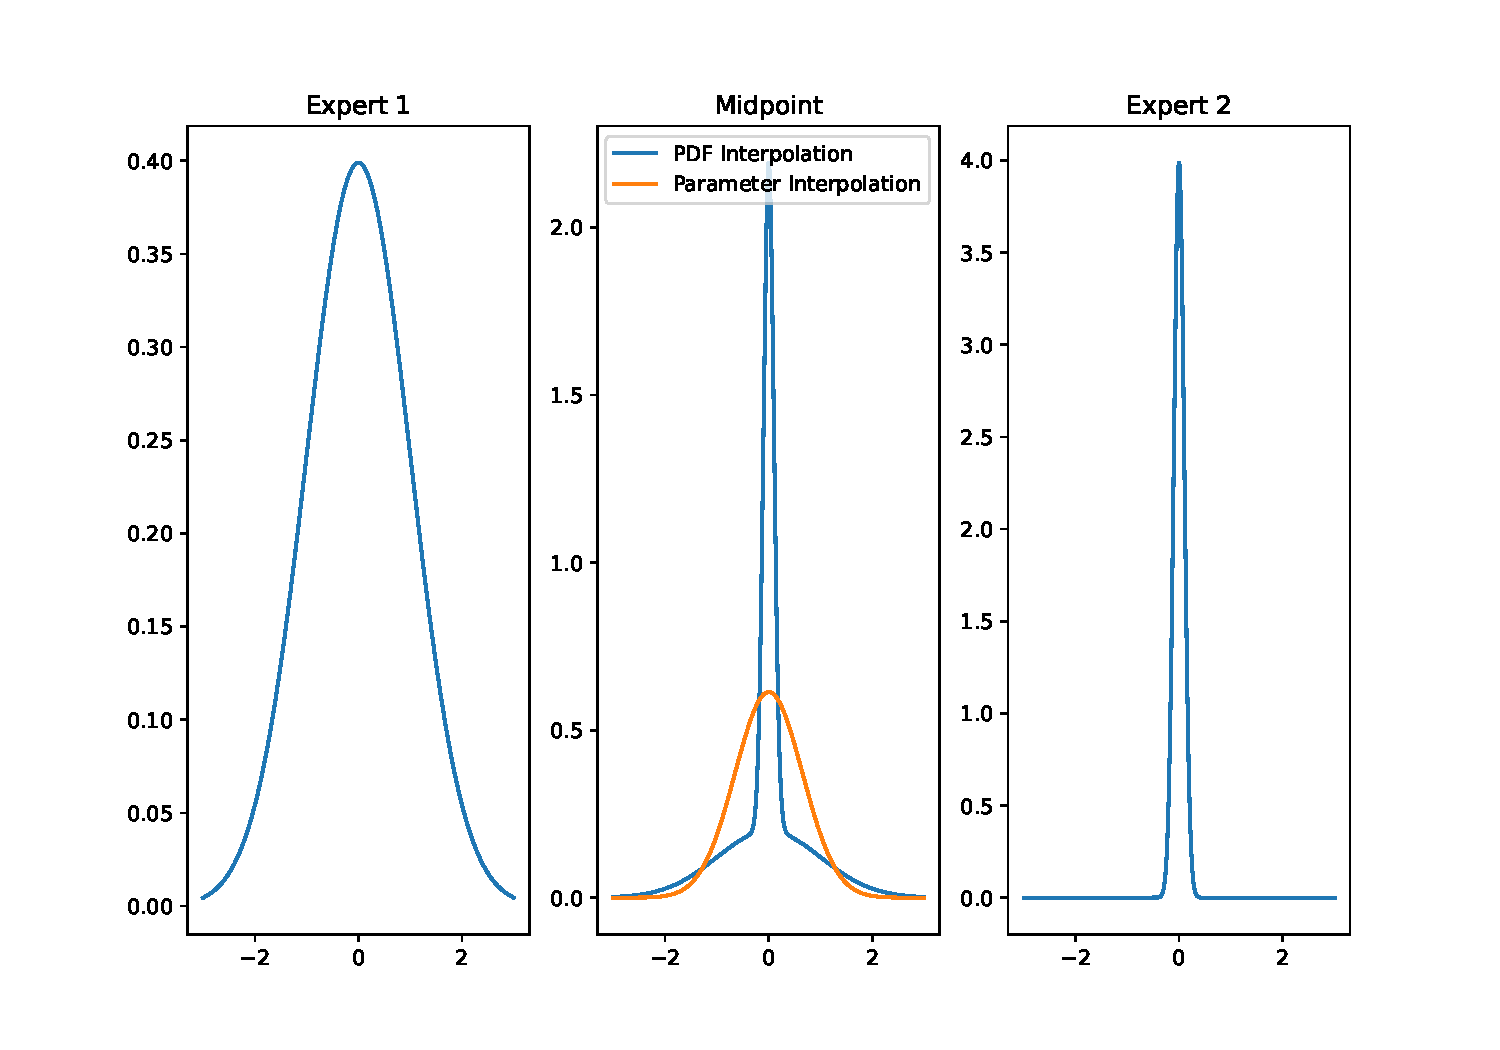
\includegraphics[width=0.9\linewidth,keepaspectratio=true]{img/merge.pdf}
			\end{center}
			\caption{An example of the two different interpolation schemes for Gaussians of differing variance}\label{F:Merge}
		\end{figure}

	\subsubsection{Interpolation Equality}

		These two methods are equal when the model is a piecewise linear (or piecewise constant) family-free\footnote{Or `non-parametric', but there are parameters!} distribution, for example:
		\begin{spalign}
			p(y|\vec{p}) & = \ell(y;\vec{p})
			\\
			&= \begin{cases}
				0                                                                                  & y \leq y_\text{min} \text{ or } y \geq y_\text{max}
				\\
				\left(p_i + \frac{(p_{i+1} - p_i)}{\Delta y}(y - y_\text{min} - i \Delta  )\right) & \text{else}
			\end{cases}
			\\
			i(y) & = \left\lfloor \frac{y - y_\text{min}}{\Delta } \right\rfloor
			\\
			p_0 & = p_{R+1} = 0
			\\
			\Delta & = \frac{y_\text{max} - y_\text{min}}{R+1}
		\end{spalign}
		This is a standard non parametric specification of a curve which is anchored to zero at the endpoints; if the parameters $\vec{p} = (p_1,...,p_R)$ are positive and normalised such that:
		\begin{equation}
			\Delta \sum_{i=1}^{R}p_i = 1
		\end{equation}
		Then this is a valid PDF. It also follows from the linearity, that:
		\begin{equation}
			\sum_i W_i p(y | \vec{p}_i) = p\left(y \left| \sum_i W_i \vec{p}_i \right.\right)
		\end{equation}
		And thus that PDFs of this form do not matter which interpolation regime is used.

	\subsubsection{The Mixed Model}

		This therefore inspires us to generate a model which has the advantages of both forms, whilst (hopefully) minimising the number of parameters. We propose that each expert in the model use a mixture model of a low-resolution family-free PDF, and a $P-$order Gaussian mixture model:

		\begin{equation}
			p(y | \vec{\xi}_i) = \sum_{j = 0}^{P-1} \pi_i^j \mathcal{N}(y; \mu_i^j, {\sigma^j_i}^2) + \pi_i^P \ell(y; \vec{p}_i)
		\end{equation}
		\def\vt{\vec{\theta}}
		Where the consensus is arrived at through Parameter interpolation, with $\vec{\Xi} = (\{\vec{\xi}_i\})$
		\begin{equation}
			\begin{split}
				p^\text{cns}(y|\vec{x},\vec{\Xi}) & = \sum_j^{P-1} \bar{\pi}_j \mathcal{N}(y; \bar{\mu}_j, \bar{\sigma^2}_j) +  \bar{\pi}_P  \ell(y; \bar{\vec{p}})
				\\
				\bar{\vec{\xi}}(\x)               & = \sum_i W_i(\x) \vec{\xi}_i
			\end{split}
		\end{equation}

\subsection{Generalised Expectation Maximisation}

	We are therefore left with a parameter vector, $\vec{\Xi}$ which is has $U = 3P + 1 + R$ dimensions (a $(\pi,\mu,\sigma^2)$ for each of the $P$ Gaussian modes, a $\pi$ for the non parametric mode, which is defined by $R$ elements). Of these $\tilde{U} = U - 2$ are independent (one degree of freedom being absorbed by the constraint $\sum_i \pi_i = 1$, and another by the constrain that $\ell$ be normalised to 1).

	Our goal is to maximise the posterior probability:
	\begin{equation}
		L(\vec{\Xi}; \mathcal{D}) =\left[ \prod_{t=0}^{T} \prod_{a = 0}^{A_t} \left(p^\text{cns}(y = y_t^a | \x_t, \vec{\Xi})\right)^{\zeta_i^a} \right]p(\vec{\Xi})
	\end{equation}
	Where we recall that we have grouped our data $\mathcal{D}$ into $N_t$ observations of $y$ for each value of the emulation parameters $\x_t$, weighted by the prior-ratio $\zeta_i^a$ (Eq. \ref{E:DefineWeights}).

	It would be possible to take derivatives with respect do $\vec{\Xi}$, but mixture models are infamously difficult to converge properly. Instead, we rely on the Generalised Expectation-Maximisation algorithm, which exhibits better convergence behaviour. This only allows us to optimise the \textit{parameters} of each expert, not their positions -- so we assume that this is handled by a separate optimisation routine.

	We assume that the experts and department positions are fixed per-iteration, and thus that $W_i(\x)$ can be computed freely: we define $W_i^t = W_i(\x_t)$ on the training data. We may then define the `complete' logarithm function associated with the latent variable $\vec{w} = (\{w_t^a\})$, which has dimensionality $D$, the total number of datapoints in the training set:
	\begin{equation}
		L(\vec{\Xi},\vec{w}) = \prod_{a,t} \prod_{p=0}^P \left[ \bar{\pi}_{p,t} f_p(y_t^a ; \bar{\vec{\theta}}_{p,t}) \right]^{\zeta_t^a \mathbb{I}(w_t^a = p)}
	\end{equation}
	Where we have defined:
	\begin{equation}
		\begin{split}
			f_p(x,\vec{\theta}_p) & = \begin{cases}
				                          \mathcal{N}(x; [\vt]_{2p}, [\vt]_{2p+1}) & 0 \leq p < P
				                          \\
				                          \ell(x; \vec{\theta})                    & p= P
			                          \end{cases}
			\\
			\text{dim}(\vt_p)     & = \begin{cases}
				                          2 & 0 \leq p < P
				                          \\
				                          R & p = P
			                          \end{cases}
			\\
			\mathbb{I}(x=y)       & = \begin{cases} 1 & x = y \\ 0 & \text{else} \end{cases}
		\end{split}
	\end{equation}
	This allows use to take the logarithm and make the mixture model separable:
	\begin{equation}
		\mathcal{L}(\vec{\Xi},\vec{w}) = \sum_{a,t,p} \mathbb{I}(w_t^a = p) \zeta_t^a\left[ \log(\bar{\pi}_{p,t}) + \log(f_p(y_t^a; \bar{\vec{\theta}}_{p,t})) \right]
	\end{equation}
	The conditional density of $\vec{w}$ - which is also known as the \textit{contribution} that each mode is making towards a give datapoint is:

	\begin{equation}
		\begin{split}
			C_{p,t,a} & = \zeta_t^a P(w_t^a = p | y_t^a, \vec{\Xi})
			\\
			          & = \zeta_t^a \frac{\bar{\pi}_{p,t} f_p(y_t^a; \bar{\vt}_{p,t})}{\sum_q\bar{\pi}_{q,t} f_q(y_t^a; \bar{\vt}_{q,t})}
		\end{split}
	\end{equation}
	We may then define the $Q$ function - the expectation of the logarithm - as:

	\begin{equation}
		\begin{split}
			Q(\vXi^\prime, \vXi) & = \int \mathrm d \vec{w} \mathcal{L}(\vXi^\prime, \vec{w}) P(\vec{w} | \vec{y}, \vXi)
			\\
			                     & = \sum_{p,t,a} C_{p,t,a}(\vXi) \left(\log(\bar{\pi}_{p,t}^\prime + \log(f_{p}(y_t^a; \bar{\vt}_{p,t}^\prime))\right)
		\end{split}
	\end{equation}
	The (G)EM algorithm relies on the statement that; given an initial set of parameters $\vXi$, a new set of parameters $\vXi^\prime$ which improves $Q$ also improves $\mathcal{L}$:
	\begin{equation}
		Q(\vXi^\prime, \vXi) \geq Q(\vXi, \vXi) \quad \Longrightarrow \quad \mathcal{L}(\vXi^\prime) \geq \mathcal{L}(\vXi)
	\end{equation}
	Given an initial guess $\vXi_0$ (and hence a set $\{C_{p,t,a}\}$ it suffices therefore to find a $\vXi^\prime$ which improves $Q$, and then set $\vXi \to \vXi^\prime$, and iterate. This is then guaranteed to converge on an optimum, and will often do so in a way which ignores many of the tight local optima that a naive gradient descent algorithm can get caught in.

	This is a standard result in mixture models: our approach is complictaed by the fact that although it is trivial to find the optimal $\bar{\pi}, \bar{\vt}$, these are not the parameters we are optimising: instead we must optimise the individual expert parameters, which are connected via:
	\begin{equation}
		\begin{split}
			\bar{\pi}_{p,t}                        & = \sum_i W_{i,t} \pi_i^p
			\\
			\bar{\mu}_{p,t}                        & = \sum_i W_{i,t} \mu_i^p
			\\
			\bar{V}_{p,t}   = \bar{\sigma^2}_{p,t} & = \sum_i W_{i,t} V_i^p
			\\
			\bar{\vec{p}}_t                        & = \sum_i W_{i,t} \vec{p}_i
		\end{split}
	\end{equation}

	However, the (G)EM approach gives us a useful starting point, because we have wrangled these quantities into \textit{separable linear terms}, which means that they can be independently maximised:
	\begin{equation}
		\begin{split}
			Q^{p}_\text{weight}(\vXi^\prime, \vXi) & = \sum_{t,a}  C_{p,t,a}(\vXi) \log(\bar{\pi}^\prime_{p,t})
			\\
			Q^{p}_\text{shape}(\vXi^\prime, \vXi)  & = \sum_{t,a} C_{p,t,a}(\vXi) \log({f}_{p}(y_t^a, \bar{\vt}_{p,t}^\prime))
		\end{split}
	\end{equation}

	\subsubsection{Iterating the Means} For $p < P$, $Q_\text{shape}^p$ is associated with the mean and variance of the Gaussian modes:

		\begin{equation}
			Q_S^p = \sum_{t,a} C_{p,t,a} \left[ -\frac{1}{2} \log(\bar{V}_{pt}) - \frac{(y_t^a - \bar{\mu}_{pt})^2}{2 \bar{V}_{pt}} \right] + \text{const}
		\end{equation}
		Then;
		\begin{equation}
			\begin{split}
				\pdiv{Q_S^p}{\mu_p^i}     & = - \left[ \underbrace{\left( \sum_{t,a} \frac{y_t^a W_{i,t} C_{p,t,a}}{\bar{V}_{p,t}} \right)}_{\vec{b}_i} - \sum_j \underbrace{\sum_{t,a} \frac{W_{i,t} W_{j,t} C_{p,t,a}}{\bar{V}_{p,t}}}_{M_{ij}} \mu_j^p \right]
				\\
				\pdiv{Q_S^p}{\vec{\mu}^p} & = - \left( \vec{b} - M \vec{\mu}^p \right)
			\end{split}
		\end{equation}
		$M$ is a Gram matrix, and thus positive definite, since $C, V > 0$. The optimal update for the means is therefore:

		\begin{equation}
			\mu^p \to M^{-1} \vec{b}
		\end{equation}

		\paragraph{Iterating the variance.} The variance is more complex, and does not have a nice simple form:
		\begin{equation}
			\pdiv{Q_S^p}{V_i^p} = \sum_{t,a} C_{p,t,a}\, W_{i,t}\left[\frac{(y_t^a-\bar\mu_{pt})^2}{2\bar V_{pt}^2} - \frac{1}{2\bar V_{pt}}\right].
		\end{equation}
		This is a concave function, but we recall that we must limit ourselves to $V_i^p > 0$ (and realistically, $V_i^p > \epsilon$, for some finite $\epsilon$). If a positive solution exists, we can reliably converge on it in a handful of Newton steps:
		\begin{equation}
			V_i^p \;\to\; V_i^p - \frac{1}{\mathcal{C}}\pdiv{Q_S^p}{V_i^p}, \qquad
			\mathcal{C} = -\sum_{t,a} C_{p,t,a}\,W_{i,t}^2\left[\frac{1}{2 \bar V_{pt}^2} \right],
		\end{equation}
		Where $\mathcal{C}$ is not the usual second derivative, but instead the Fisher Scoring derivative, which guarantees each step is in the right direction, at the cost of slightly slower convergence.
		\paragraph{Iterating the Weights} The values of $(\mu, V)$ were coupled across a single mode; we evaluated one mode at a time, of all the experts. The weights are different, as they are coupled across an expert by the requirement that they sum to one. We will therefore update the block $\vec{\pi}_i = \left(\pi_i^0, \pi_i^1, ... \pi_i^{P-1} \right)$. In order to update the weights, we have to repeat the initial E-M trick, by introducing the contribution that each expert is providing to the overall weight:
		\begin{equation}
			s_{j,t,p} = \frac{W_{j,t}\,\pi_{j}^p}{\bar\pi_{p,t}} = \frac{W_{j,t} \pi_j^p}{\sum_i W_{i,t} \pi_i^p}
		\end{equation}
		We then average this over all the data points:
		\begin{equation}
			[\vec{c}_{j}]_p = \sum_{t,a}C_{p,t,a}\,s_{j,t,p},
		\end{equation}
		Providing a simple update rule:
		\begin{equation}
			\vec{\pi}_{j} \;\leftarrow\; \frac{\vec{c}_{j}}{ \vec{c}_{j} \cdot \vec{1}}.
		\end{equation}
		We do note that this \textit{doesn't} provide the optimal set of $\vec{\pi}_j$; but it is guaranteed to be \textit{better than the previous guess}. This is why we are using the \textit{Generalised}-EM algorithm; we are not perfectly optimising $\vXi^\prime$, merely improving it, which is a sufficient condition to converge on an optimum.

		\paragraph{Iterating the non-parametric parameters} The final element is to determine the update rule for $\vec{p}_i$, the low resolution non-parametric mode. This has an almost identical form to the update rule for the weights, defining a per-bin contribution, with the only major difference being that $r$ only has a contribution if $y_- \leq y_t^a < y_+$; i.e. it lies within the linear interpolation region that the parameter is associated with.

		\begin{equation}
			r_{j,t,k}(y) = \frac{W_{j,t}\,c_k(y)\,p_j^k}{\sum_{k^\prime} c_{k^\prime}(y)\,\bar p^{k^\prime}_t}, \qquad c_k(y) = \begin{cases}1-\frac{y-y_\text{min}-i(y)\Delta}{\Delta} & k=i(y)\\ \frac{y-y_\text{min}-i(y)\Delta}{\Delta} & k=i(y)+1\\ 0 &\text{else}\end{cases}
		\end{equation}
		Then:
		\begin{equation}
			[\vec{u}_j]_k =  \sum_{t,a} C_{{P-1},t,a} \times r_{j,t,k} (y_t^a)
		\end{equation}
		And finally:
		\begin{equation}
			\vec{p}_i \to \Delta^{-1} \frac{\vec{u}_i}{\vec{u}_i \cdot \vec{1}}
		\end{equation}

		\begin{aside}[Not implemented!]
			Note that as of 3/8/26, the non-parametric baseline is not implemented within the code.
		\end{aside}

\subsection{Priors}

	We mentioned priors earlier, and then omitted them when doing the EM. Priors \textit{can} be included in the EM algorithm, but it is less convenient than in a basic gradient descent.

	The Variance, however, is pretty easy (since that does compute the gradient and take optimisation steps). Imposing an inverse gamma prior on $V_{i,p}$ during these steps prevents the variance crashing to zero.
	% 	\clearpage
	%
	%
	%
	%
	%
	%
	%
	%
	%
	%
	%
	%



